\documentclass{ltxdoc}
\usepackage[show]{cloze}
\usepackage{graphicx}
\usepackage{paralist}
\usepackage{forest}
\usepackage{multicol}
\usepackage{tikz}
\usetikzlibrary{positioning}

%%
% titlesec
%%

\usepackage{titlesec}
\titleformat{\paragraph}[hang]{%
  \normalfont\normalsize\bfseries%
  }{\theparagraph}{1em}{}
\titleformat{\subparagraph}[hang]{%
  \normalfont\small\bfseries%
  }{\thesubparagraph}{1em}{}
  \titlespacing*{\subparagraph}{0pt}{*1}{0pt}

%%
% hyperref
%%

\usepackage[
  colorlinks=true,
  linkcolor=red,
  filecolor=red,
  urlcolor=red,
]{hyperref}

%%
% mdframed
%%

\usepackage{mdframed}
\definecolor{TmpGray}{gray}{0.95}
% f2d6aa 242 214 170
\definecolor{TmpYellow}{rgb}{0.949019608, 0.839215686, 0.666666667}
\newmdenv[
  backgroundcolor=TmpYellow!3,
  linecolor=TmpYellow!70
]{TmpExample}
\surroundwithmdframed[backgroundcolor=TmpGray]{verbatim}

%%
% minted
%%

\usepackage{minted}
\usemintedstyle{colorful}
\BeforeBeginEnvironment{minted}{\begin{mdframed}[
  backgroundcolor=TmpGray!60,
  linecolor=gray!40,
]}
\AfterEndEnvironment{minted}{\end{mdframed}}
\setminted{
  breaklines=true,
  fontsize=\footnotesize,
}

\MakeShortVerb{\|}

%%
% Temporary local macros
%%

\newcommand{\TmpExpDesc}[1]{(|#1|)}

\newcommand{\TmpDesc}[1]{%
  \hfill%
  \TmpExpDesc{#1}%
  \par%
}

\def\tt#1{%
  \texttt{#1}%
}

\def\TmpSecRef#1{%
  (\rightarrow\ \ref{#1})%
}

\def\TmpOption#1#2{%
  \tt{[#1=}\meta{#2}\tt{]}%
}

\def\TmpHide{%
  \noindent%
  \texttt{\string\clozehide}:%
  \clozehide%
}

\def\TmpShow{%
  \noindent%
  \texttt{\string\clozeshow}:%
  \clozeshow%
}

\def\TmpReduceVspace{%
  \vspace{-0.2cm}%
}

\EnableCrossrefs
\CodelineIndex
\RecordChanges
\begin{document}

%%%%%%%%%%%%%%%%%%%%%%%%%%%%%%%%%%%%%%%%%%%%%%%%%%%%%%%%%%%%%%%%%%%%%%%%
%
%%%%%%%%%%%%%%%%%%%%%%%%%%%%%%%%%%%%%%%%%%%%%%%%%%%%%%%%%%%%%%%%%%%%%%%%

\providecommand*{\url}{\texttt}
\GetFileInfo{cloze.dtx}
\title{The \cloze{cloze} package%
  \thanks{Many thanks to Robert-Michael Huber for his advice
and to Paul Isambert for his article \emph{"Three things you can do with
Lua\TeX{} that would be extremely painful otherwise"} in TUGboat, Volume
31 (2010), No. 3. This article helped a lot to write this package.}%
}
\author{%
  Josef Friedrich\\%
  \url{josef@friedrich.rocks}\\%
  \href{https://github.com/Josef-Friedrich/cloze}
  {github.com/Josef-Friedrich/cloze}%
}
\date{v1.6~from 2020/06/30}

\maketitle\vfill

\pagebreak

\setcounter{secnumdepth}{5}
\setcounter{tocdepth}{5}
\tableofcontents

%-----------------------------------------------------------------------
% Introduction
%-----------------------------------------------------------------------

\pagebreak
\section{Introduction}

\emph{cloze} is a plain \TeX{} or a \LaTeX{} package to generate cloze
texts. It uses the capabilities of the modern \TeX{} engine
\emph{Lua\TeX}. Therefore, you must use Lua\TeX{} or Lua\LaTeX{} to
create documents containing gaps.

\begin{center}
\begin{minipage}{0.4\linewidth}
\begin{verbatim}
lualatex cloze-text.tex
\end{verbatim}
\end{minipage}
or
\begin{minipage}{0.4\linewidth}
\begin{verbatim}
luatex cloze-text.tex
\end{verbatim}
\end{minipage}
\end{center}

\noindent
The main feature of the package is that the formatting doesn't change
when using the |hide| and |show| \TmpSecRef{sec:option-hide} options.

\newcommand{\clozelorem}{%
Lorem ipsum \cloze{dolor sit} amet, consectetur \cloze{adipisicing}
elit, sed do eiusmod tempor incididunt ut labore et \cloze{dolore magna}
aliqua. Ut enim ad minim veniam, quis nostrud \cloze{exercitation}
ullamco laboris nisi ut \cloze{aliquip} ex ea commodo consequat.%
}

\begin{TmpExample}
\clozelorem
\end{TmpExample}

\clozeset{hide}

\noindent
The command |\clozeset{hide}| only shows gaps. When you put both texts
on top of each other you will see that they perfectly match.

\begin{TmpExample}
\clozelorem
\end{TmpExample}

\clozeset{show}

%-----------------------------------------------------------------------
% Usage
%-----------------------------------------------------------------------

\section{Usage}

%-----------------------------------------------------------------------
%
%-----------------------------------------------------------------------

\subsection{Interfaces}

The main difference between the plain \TeX{} and the \LaTeX{} interface
is option handling. In \LaTeX{} options can be set by using key-value
pairs. In plain \TeX{} the only possibility to set options is to use the
macro \cmd{\clozesetoption} \TmpSecRef{sec:command-clozesetoption}.

%%
%
%%

\subsubsection{The plain \TeX{} interface}

\begin{minted}{tex}
\input cloze.tex
\clozesetoption{margin}{1cm}
\clozeshow
Lorem \cloze{ipsum} dolor.
\bye
\end{minted}

%%
%
%%

\subsubsection{The \LaTeX{} interface}

\begin{minted}{latex}
\documentclass{article}
\usepackage[show,margin=1cm]{cloze}
\begin{document}
Lorem \cloze{ipsum} dolor.
\end{document}
\end{minted}

\subsection{The commands and environments}

There are the commands
\cmd{\cloze},
\cmd{\clozefix},
\cmd{\clozefil},
\cmd{\clozenol},
\cmd{\clozeparcmd},
\cmd{\clozestrike} and the environments
|clozepar| and
|clozebox|
to generate cloze texts.

%%
% \cloze
%%

\subsubsection{\cmd{\cloze}}
\label{sec:command-cloze}

\DescribeMacro{\cloze} \cmd{\cloze}\oarg{options}\marg{some text}: The
command \cmd{\cloze} is similar to a command that offers the possibility
to underline the texts. \cmd{\cloze} does not prevent line breaks. The
width of a gap depends on the number of letters and the font used.
The only option which affects the widths of a gap is the option
|margin| \TmpSecRef{sec:option-margin}.

\begin{TmpExample}
Lorem ipsum \cloze{dolor} sit amet, \cloze{consectetur} adipisicing
elit, sed do eiusmod tempor incididunt ut labore et dolore
\cloze{magna aliqua. Ut enim ad minim veniam, quis nostrud exercitation
ullamco laboris nisi} ut aliquip ex ea commodo consequat.
\end{TmpExample}

\noindent It is possible to convert a complete paragraph into a `gap'.
But don't forget: There is a special environment for this: \tt{clozepar}
\TmpSecRef{sec:command-clozepar}.

\begin{TmpExample}
\cloze{Lorem ipsum dolor sit amet, consectetur adipisicing elit, sed do
eiusmod tempor incididunt ut labore et dolore magna aliqua. Ut enim ad
minim veniam, quis nostrud exercitation ullamco laboris nisi ut aliquip
ex ea commodo consequat.}
\end{TmpExample}

\noindent The command \cmd{\cloze} doesn't change the behavior of the
hyphenation. Let's try some long German words:

\begin{TmpExample}
es
\cloze{Te\-le\-kom\-mu\-ni\-ka\-tions\-ü\-ber\-wach\-ung}
geht
\cloze{Un\-ter\-neh\-mens\-steu\-er\-fort\-ent\-wick\-lungs\-ge\-setz}
\cloze{Ab\-teil\-ungs\-lei\-ter\-in}
\cloze{Ober\-kom\-mi\-sar\-in}
auch
\cloze{Fil\-lial\-lei\-ter\-in}
kurz.
\end{TmpExample}

%%
% \clozesetfont
%%

\subsubsection{\cmd{\clozesetfont}}
\label{sec:command-clozesetfont}
\label{sec:command-clozefont}

\DescribeMacro{\clozesetfont}
The gap font can be changed by using the command
\cmd{\clozesetfont}. \tt{\string\cloze\-set\-font} redefines the command
\cmd{\clozefont} which contains the font definition.
Thus, the command \tt{\string\clozesetfont\string{\string\Large\string}}
has the same effect as
|\def\clozefont{\Large}|

\clozesetfont{\Large}

\begin{TmpExample}
Excepteur \cloze{sint} occaecat \cloze{cupidatat} non proident.
\end{TmpExample}

\noindent Please do not put any color definitions in
\cmd{\clozesetfont}, as it won't work. Use the option
|textcolor| instead \TmpSecRef{sec:option-textcolor}.

|\clozesetfont{\ttfamily\normalsize}| changes the gap text for example
into a normal sized typewriter font.

\clozesetfont{\ttfamily\normalsize}

\begin{TmpExample}
Excepteur \cloze{sint} occaecat \cloze{cupidatat} non proident.
\end{TmpExample}

\clozesetfont{\itshape}

%%
% \clozefix
%%

\subsubsection{\cmd{\clozefix}}
\label{sec:command-clozefix}

\DescribeMacro{\clozefix} \cmd{\clozefix}\oarg{options}\marg{some text}:
The command \cmd{\clozefix} creates gaps with a fixed width. The
clozes are default concering the width \tt{\ClozeGetOption{width}}.

\begin{TmpExample}
\noindent Lorem ipsum dolor sit amet:
\begin{compactenum}
\item \clozefix[width=5cm]{consectetur}
\item \clozefix[width=5cm]{adipisicing}
\item \clozefix[width=5cm]{elit}
\end{compactenum}
sed do eiusmod.
\end{TmpExample}

Gaps with a fixed width are much harder to solve.

\begin{TmpExample}
Lorem ipsum dolor \clozefix[align=center,width=3cm]{sit} amet,
\clozefix[align=center,width=3cm]{consectetur} adipisicing elit, sed do
eiusmod tempor incididunt \clozefix[align=center,width=3cm]{ut} labore
et dolore magna aliqua.
\end{TmpExample}

Using the option |align| you can make nice tabulars like this:

\begin{TmpExample}
\begin{tabular}{p{5cm}p{4cm}}
\raggedleft Composer & Life span \\

\clozefix[width=5cm,align=right]{Joseph Haydn} &
\clozefix{1723-1809} \\

\clozefix[width=5cm,align=right]{Wolfgang Amadeus Mozart} &
\clozefix{1756-1791} \\

\clozefix[width=5cm,align=right]{Ludwig van Beethoven} &
\clozefix{1770-1827} \\
\end{tabular}
\end{TmpExample}

%%
% \clozenol
%%

\subsubsection{\cmd{\clozenol}}
\label{sec:command-clozenol}
\DescribeMacro{\clozenol} \cmd{\clozenol}\oarg{options}\marg{some text}:
The macro name |clozenol| stands for \emph{“cloze no line”}. As the
the name suggests this macro typesets cloze texts without a line.
\cmd{\clozenol} is a convenient abbreviation for
|\cloze[thickness=0pt]{text}|.

\begin{minted}{latex}
Lorem \clozenol{ipsum dolor} sit amet.
\end{minted}

\begin{TmpExample}
Lorem \clozenol{ipsum dolor} sit amet.
\end{TmpExample}

\begin{minted}{latex}
Lorem \clozenol[textcolor=green]{ipsum dolor} sit amet.
\end{minted}

\begin{TmpExample}
Lorem \clozenol[textcolor=green]{ipsum dolor} sit amet.
\end{TmpExample}

\noindent
The next examples are showing that \cmd{\clozenol} behaves exactly as
\cmd{\clozenol} with the option |thickness=0pt|
(|\cloze[thickness=0pt]|) set: The text layout doesn’t change if we are
hiding the gaps and the hidden text is not really hidden. It is removed.
It can not be copied.

\begin{mdframed}[backgroundcolor=gray!40]
Lorem ipsum \clozenol{dolor sit amet, consetetur sadipscing elitr, sed
diam nonumy eirmod tempor invidunt ut labore et dolore magna aliquyam
erat, sed diam voluptua} sit amet.
\end{mdframed}

\noindent
Now hide the text

\clozehide

\begin{mdframed}[backgroundcolor=gray!40]
Lorem ipsum \clozenol{dolor sit amet, consetetur sadipscing elitr, sed
diam nonumy eirmod tempor invidunt ut labore et dolore magna aliquyam
erat, sed diam voluptua} sit amet.
\end{mdframed}

\clozeshow

%%
% \clozefil
%%

\subsubsection{\cmd{\clozefil}}
\label{sec:command-clozefil}

\DescribeMacro{\clozefil} \cmd{\clozefil}\oarg{options}\marg{some text}:
The name of the command is inspired by \cmd{\hfil}, \cmd{\hfill}, and
\cmd{\hfilll}. Only \cmd{\clozefil} fills out all available horizontal
spaces with a line.

\begin{TmpExample}
Lorem ipsum dolor sit amet, \clozefil{consectetur adipisicing elit, sed
do eiusmod.}

Ut enim \clozefil{ad minim veniam} exercitation.
\end{TmpExample}

%%
% \clozeextend
%%

\subsubsection{\cmd{\clozeextend}}
\label{sec:command-clozeextend}

\DescribeMacro{\clozeextend} \cmd{\clozeextend}\oarg{spaces}:
The command |\clozeextend| adds some invisible placeholders to extend
some cloze texts with blank space.

\begin{minted}{latex}
\begin{itemize}
\item \clozefil{Lorem ipsum dolor sit amet, consectetur adipisicing
elit, sed do eiusmod tempor incididunt ut labore et dolore magna
aliqua.}
\item \clozefil{Ut enim ad minim veniam \clozeextend[20]}
\item \clozefil{quis nostrud \clozeextend[20]}
\end{itemize}
\end{minted}

\begin{TmpExample}
\begin{itemize}
\item \clozefil{Lorem ipsum dolor sit amet, consectetur adipisicing
elit, sed do eiusmod tempor incididunt ut labore et dolore magna
aliqua.}
\item \clozefil{Ut enim ad minim veniam \clozeextend[20]}
\item \clozefil{quis nostrud \clozeextend[20]}
\end{itemize}
\end{TmpExample}

%%
% clozepar
%%

\subsubsection{\tt{clozepar}}
\label{sec:command-clozepar}

\DescribeEnv{clozepar} |\begin{clozepar}|\oarg{options} \dots
\textit{some text} \dots |\end{clozepar}|: The environment \tt{clozepar}
transforms a complete paragraph into a cloze text. The options |align|,
|margin| and |width| have no effect on this environment.

\begin{TmpExample}
Lorem ipsum dolor sit amet, consectetur adipisicing elit ullamco laboris
nisi.

\begin{clozepar}
Ut enim ad minim veniam, quis nostrud exercitation ullamco laboris nisi
ut aliquip ex ea commodo consequat. Duis aute irure dolor in
reprehenderit in voluptate velit esse cillum.
\end{clozepar}

Excepteur sint occaecat cupidatat non proident.
\end{TmpExample}

%%
% \clozeparcmd
%%

\subsubsection{\cmd{\clozeparcmd}}
\label{sec:command-clozeparcmd}
\DescribeMacro{\clozeparcmd} \cmd{\clozeparcmd}: The command
\cmd{\clozeparcmd} is the macro version of the environment |clozepar|.

%%
% clozebox
%%

\subsubsection{\tt{clozebox}}
\label{sec:command-clozebox}

\DescribeEnv{clozebox} |\begin{clozebox}|*\oarg{options} \dots
\textit{some text} \dots |\end{clozebox}|: The environment \tt{clozebox}
surrounds a text with a box. The starred version omits the line around
the box. Use the options |boxwidth| and |boxheight| to specify the
dimensions of the box. By default the width of the box is |\linewidth|.
The height of the box is determined by the amount of text. This
environment is realized by a combination of the |minipage| environment
surrounded by a \cmd{\fbox}. For the cloze text the macro
\cmd{\clozenol} is reused. New paragraphs are not allowed inside a cloze
box. Use two backslashes multiple times |\\| instead.

\begin{minted}{latex}
\begin{clozebox}
Lorem ipsum dolor sit amet, consectetur adipisicing elit, sed do eiusmod
tempor incididunt ut labore et dolore magna aliqua.
\end{clozebox}
\end{minted}

\noindent
\begin{minipage}{0.4\linewidth}
\noindent
|\clozehide|
\clozehide
\bigskip
\begin{clozebox}
Lorem ipsum dolor sit amet, consectetur adipisicing elit, sed do eiusmod
tempor incididunt ut labore et dolore magna aliqua.
\end{clozebox}
\end{minipage}
\hfil
\begin{minipage}{0.4\linewidth}
\noindent
|\clozeshow|
\clozeshow
\bigskip
\begin{clozebox}[margin=0pt]
Lorem ipsum dolor sit amet, consectetur adipisicing elit, sed do eiusmod
tempor incididunt ut labore et dolore magna aliqua.
\end{clozebox}
\end{minipage}

\noindent
Like with all cloze macros and environments the hidden text vanishes
from the rendered file. The next example demonstrates this by showing a
different background color:

\def\TmpClozeBox{
  \bigskip
  \begin{center}
  \begin{clozebox}[boxwidth=4cm]
  Lorem ipsum dolor sit amet.
  \end{clozebox}
  \end{center}
  \bigskip
}

\begin{multicols}{2}

\TmpHide
\begin{TmpExample}
\TmpClozeBox
\end{TmpExample}

\TmpShow
\begin{TmpExample}
\TmpClozeBox
\end{TmpExample}
\end{multicols}

\paragraph{Option boxwidth}
\label{sec:command-clozebox-boxwidth}
See the documentation about the option \TmpSecRef{sec:option-boxwidth}.

\begin{minted}{latex}
\begin{clozebox}[boxwidth=5cm]
\end{minted}

\begin{TmpExample}
\bigskip
\begin{center}
\begin{clozebox}[boxwidth=2.5cm]
boxwidth: 2.5cm; Lorem ipsum dolor sit amet ...
\end{clozebox}
\begin{clozebox}[boxwidth=3cm]
boxwidth: 3cm; Lorem ipsum dolor sit amet ...
\end{clozebox}
\begin{clozebox}[boxwidth=5cm]
boxwidth: 4cm; Lorem ipsum dolor sit amet ...
\end{clozebox}
\end{center}
\bigskip
\end{TmpExample}

\paragraph{Option boxheight}
\label{sec:command-clozebox-boxheight}
See the documentation about the option \TmpSecRef{sec:option-boxheight}.

\begin{minted}{latex}
\begin{clozebox}[boxheight=3cm]
\end{minted}

\TmpReduceVspace

\begin{TmpExample}
\bigskip
\begin{center}
\begin{clozebox}[boxheight=3cm,boxwidth=3cm]
boxheight: 3cm; Lorem ipsum dolor sit amet ...
\end{clozebox}
\begin{clozebox}[boxheight=2cm,boxwidth=3cm]
boxheight: 2cm; Lorem ipsum dolor sit amet ...
\end{clozebox}
\begin{clozebox}[boxheight=1cm,boxwidth=3cm]
boxheight: 1cm; Lorem ipsum dolor sit amet ...
\end{clozebox}
\end{center}
\bigskip
\end{TmpExample}

\paragraph{starred}

The starred version omits the line around the box.

% starred

\begin{minipage}[t]{0.55\linewidth}
\begin{minted}{latex}
\begin{clozebox}*[boxheight=5cm]
Lorem ...
\end{clozebox}
\end{minted}
\end{minipage}
%
\begin{minipage}[t]{0.4\linewidth}
\begin{TmpExample}
\begin{center}
\begin{clozebox}*[boxwidth=4cm,boxheight=3cm]
Lorem ipsum dolor sit amet, consectetur adipisicing elit, sed do eiusmod
tempor incididunt ut labore et dolore magna aliqua.
\end{clozebox}
\end{center}
\end{TmpExample}
\end{minipage}

%%
% clozespace
%%

\subsubsection{\tt{clozespace}}
\label{sec:command-clozespace}

\DescribeEnv{clozespace} |\begin{clozespace}|\oarg{options} \dots
\textit{some text} \dots |\end{clozespace}|: If you are using a
bigger font for the cloze text as for the normal text, you are getting
irregular distances between the lines:

\def\TmpOrbit{
\clozesetfont{\Huge\fontspec{Kalam}}
Today in the Discovery Lab we learned about three types of spacecraft
that are helping us explore \cloze{Mars}. The \cloze{spacecraft} are on
Mrs. Bratt’s Principal’s Reading Challenge board. One type of spacecraft
is the \cloze{orbiter}.
}

\begin{minted}{latex}
\clozesetfont{\Huge\fontspec{Kalam}}
Today in the Discovery ...
\end{minted}
\TmpReduceVspace
% https://en.wikipedia.org/wiki/Cloze_test#/media/File:Student_matching_cloze_terms_on_smartboard.jpg
\begin{TmpExample}
\TmpOrbit
\end{TmpExample}

\noindent
With the environment |clozespace| you are able to restore the regular
balanced line spacing. The default value for the option |spacing| is
\tt{\ClozeGetOption{spacing}}. Also take a look in the section about the
option |spacing| \TmpSecRef{sec:option-spacing}.

\begin{minted}{latex}
\begin{clozespace}[spacing=2]
...
\end{clozespace}
\end{minted}
\TmpReduceVspace
\begin{TmpExample}
\begin{clozespace}[spacing=2]
\TmpOrbit
\end{clozespace}
\TmpReduceVspace
\end{TmpExample}

\noindent
The environment |clozespace| uses the package
\href{https://www.ctan.org/pkg/setspace}{setspace} in the background for
setting the spacing between the lines.

%%
% \clozeline
%%

\subsubsection{\cmd{\clozeline}}
\label{sec:command-clozeline}

\DescribeMacro{\clozeline}
%
\cmd{\clozeline}\oarg{options}: To create a cloze line of a certain
width, use the command \cmd{\clozeline}. The default width of the line
is \tt{\ClozeGetOption{width}}. In combination with the other cloze
commands you can create for example an irregular alignment of the cloze
text.

\begin{minted}{latex}
Ut enim ad
\clozeline[width=1cm]\cloze{minim}\clozeline[width=3cm]
minim veniam
\end{minted}

\begin{TmpExample}
Ut enim ad \clozeline[width=1cm]\cloze{minim}\clozeline[width=3cm] minim
veniam,
\end{TmpExample}

%%
% \clozelinefil
%%

\subsubsection{\cmd{\clozelinefil}}
\label{sec:command-clozelinefil}

\DescribeMacro{\clozelinefil}
\cmd{\clozelinefil}\oarg{options}:
This command \cmd{\clozelinefil} fills the
complete available horizontal space with a line. Moreover,
\cmd{\clozelinefil} was used to create \cmd{\clozefil}.

\begin{TmpExample}
Lorem\clozelinefil
\end{TmpExample}

%%
% \clozestrike
%%

\subsubsection{\cmd{\clozestrike}}
\label{sec:command-clozelinefil}

\DescribeMacro{\clozestrike}
\cmd{\clozestrike}\oarg{options}\marg{wrong text}\marg{correct text}:
This macro can be useful for worksheets that contain intentionally
errors. The pupils have to find and cross out the mistakes and
write the right solution on top of the errors.

\begin{minted}{latex}
Wolfgang Amadeus Mozart was born in \clozestrike{Vienna}{Salzburg}.
\end{minted}

\begin{TmpExample}
Wolfgang Amadeus Mozart was born in \clozestrike{Vienna}{Salzburg}.
\end{TmpExample}

\noindent
The option |linecolor| has no effect on the lines produced by the
macro \cmd{\clozestrike}. The line color and and the text color
are both the same, because the pupils have to draw the lines.

\begin{minted}{latex}
Mozart’s father was called
\clozestrike[textcolor=red]{Ludwig}{Leopold} Mozart.
\end{minted}

\begin{TmpExample}
Mozart’s father was called
\clozestrike[textcolor=red]{Ludwig}{Leopold} Mozart.
\end{TmpExample}

%-----------------------------------------------------------------------
% Options
%-----------------------------------------------------------------------

\subsection{The options}

%%
% Local and global options
%%

\subsubsection{Local and global options}

The \emph{cloze} package distinguishs between \emph{local} and
\emph{global} options. Besides the possiblity to set \emph{global}
options in the \cmd{\usepackage}\oarg{global options}\marg{cloze}
declaration, the cloze package offers a special command to set
\emph{global} options:
\cmd{\clozeset}\marg{global options}

%%
% \clozesetoption
%%

\subsubsection{\cmd{\clozesetoption}}
\label{sec:command-clozesetoption}

\DescribeMacro{\clozesetoption}
\cmd{\clozesetoption}\marg{key}\marg{value}: Set a single option. In
plain \TeX{} the command sets the options only in the global option
space.

%%
% \clozeset
%%

\subsubsection{\cmd{\clozeset}}
\label{sec:command-clozeset}

\DescribeMacro{\clozeset}
\cmd{\clozeset}\marg{global options}: The command can set \emph{global}
options for each paragraph.

\begin{minted}{latex}
\clozeset{textcolor=red} Lorem \cloze{ipsum} dolor \par
\clozeset{textcolor=green} Lorem \cloze{ipsum} dolor
\end{minted}

\begin{TmpExample}
\clozeset{textcolor=red} Lorem \cloze{ipsum} dolor \par
\clozeset{textcolor=green} Lorem \cloze{ipsum} dolor
\end{TmpExample}

\noindent \cmd{\clozeset} does not change the options within a
paragraph. As you can see in the example below the last \cmd{\clozeset}
applies the color green for both gaps.

\begin{minted}{latex}
\clozeset{textcolor=red} Lorem \cloze{ipsum} dolor
\clozeset{textcolor=green} Lorem \cloze{ipsum} dolor
\end{minted}

\begin{TmpExample}
\clozeset{textcolor=red} Lorem \cloze{ipsum} dolor
\clozeset{textcolor=green} Lorem \cloze{ipsum} dolor
\end{TmpExample}

\clozereset

%%
% \clozereset
%%

\subsubsection{\cmd{\clozereset}}
\label{sec:command-clozereset}

\DescribeMacro{\clozereset}
\cmd{\clozereset}: The command resets all \emph{global} options to the
default values. It has no effect on the \emph{local} options.

\begin{minted}{latex}
\clozeset{
  thickness=3mm,
  linecolor=yellow,
  textcolor=magenta,
  margin=-2pt
}
\end{minted}

\clozeset{thickness=3mm,linecolor=yellow,textcolor=magenta,margin=-2pt}

\begin{TmpExample}
Very \cloze{silly} global \cloze{options}.
\end{TmpExample}

\begin{minted}{latex}
\clozereset
\end{minted}
\clozereset

\begin{TmpExample}
\cloze{Relax!} We can reset \cloze{those} options.
\end{TmpExample}

%%
% \clozereset
%%

\subsubsection{\cmd{\clozeshow} and \cmd{\clozehide}}
\label{sec:command-clozeshow}
\label{sec:command-clozehide}

\DescribeMacro{\clozeshow} \DescribeMacro{\clozehide}
\cmd{\clozeshow} and \cmd{\clozehide}: This commands are shortcuts for
\cmd{\clozeset}\marg{show} and \cmd{\clozeset}\marg{hide}.

\begin{minted}{latex}
\clozehide
\end{minted}
\clozehide

\begin{TmpExample}
Lorem \cloze{ipsum dolor sit} amet, consectetur \cloze{adipisicing}
elit.
\end{TmpExample}

\begin{minted}{latex}
\clozeshow
\end{minted}
\clozeshow

\begin{TmpExample}
Lorem \cloze{ipsum dolor sit} amet, consectetur \cloze{adipisicing}
elit.
\end{TmpExample}

%%
% align
%%

\subsubsection{\tt{align}}
\label{sec:option-align}

\TmpOption{align}{left/center/right}:
%
Only the macro \cmd{\clozefix} \TmpSecRef{sec:command-clozefix} takes
the option \tt{align} into account. Possible values are \tt{left},
\tt{center} and \tt{right}. This option only makes sense, if the width
of the line is larger than the width of the text.

\newcommand{\TmpOptionsalign}[1]{%
  \noindent%
  \clozefix[align=#1,width=8cm]{Lorem ipsum}%
  \TmpDesc{#1}%
}

\begin{TmpExample}
\TmpOptionsalign{left}
\TmpOptionsalign{center}
\TmpOptionsalign{right}
\end{TmpExample}

%%
% boxheight
%%

\subsubsection{\tt{boxheight}}
\label{sec:option-boxheight}

|boxheight| specifies the height of a cloze box. This option has only
an effect on the environment |clozebox| \TmpSecRef{sec:command-clozebox}.
An example can be found in the section about the environment
\TmpSecRef{sec:command-clozebox-boxheight}.

%%
% boxwidth
%%

\subsubsection{\tt{boxwidth}}
\label{sec:option-boxwidth}

|boxwidth| specifies the width of a cloze box. This option has only an
effect on the environment |clozebox| \TmpSecRef{sec:command-clozebox}.
An example can be found in the section about the environment
\TmpSecRef{sec:command-clozebox-boxwidth}.

%%
% distance
%%

\subsubsection{\tt{distance}}
\label{sec:option-distance}

\TmpOption{distance}{dimen}:
The option |distance| specifies the spacing between the baseline of the
text and the gap line. The larger the dimension of the option
|distance|, the more moves the line down. Negative values cause the line
to appear above the baseline. The default value is
\tt{\ClozeGetOption{distance}}.

\newcommand{\TmpOptiondistance}[1]{%
  \noindent%
  \clozefil[distance=#1]{Lorem ipsum dolor sit amet.}
  \TmpExpDesc{#1}
  \par%
}

\begin{TmpExample}
\TmpOptiondistance{\ClozeGetOption{distance}}
\TmpOptiondistance{3pt}
\TmpOptiondistance{-3pt}
\end{TmpExample}

%%
% hide and show
%%

\subsubsection{\tt{hide} and \tt{show}}
\label{sec:option-hide}
\label{sec:option-show}

\tt{[hide]} and \tt{[show]}:
By default the cloze text is displayed. Use the option |hide| to remove
the cloze text from the output.  If you accidentally specify both
options -- |hide| and |show| -- the last option "wins".

\newcommand{\TmpOptionshow}[1]{%
  \noindent%
  Lorem ipsum \cloze[#1]{dolor sit amet}, consectetur
  \cloze[#1]{adipisicing} elit.%
  \TmpDesc{#1}%
}

\begin{TmpExample}
\TmpOptionshow{hide}
\TmpOptionshow{show}
\TmpOptionshow{show,hide}
\TmpOptionshow{hide,show}
\end{TmpExample}

%%
% linecolor and textcolor
%%

\subsubsection{\tt{linecolor} and \tt{textcolor}}
\label{sec:option-linecolor}
\label{sec:option-textcolor}

\TmpOption{linecolor}{color name} and
\TmpOption{textcolor}{color name}:
Values for both color options are color names used by the xcolor
package. To define your own color use the following command:

\begin{minted}{latex}
\definecolor{myclozecolor}{rgb}{0.1,0.4,0.6}
\cloze[textcolor=myclozecolor]{Lorem ipsum}
\end{minted}
\definecolor{myclozecolor}{rgb}{0.1,0.4,0.6}

\newcommand{\TmpOptioncolor}[2]{%
  \noindent%
  \clozefil[#1=#2]{Lorem ipsum dolor sit amet, consectetur} %
  \TmpExpDesc{#2}%
  \par%
}

\begin{TmpExample}
\TmpOptioncolor{textcolor}{myclozecolor}
\TmpOptioncolor{textcolor}{red}
\TmpOptioncolor{textcolor}{green}
\end{TmpExample}

\noindent You can use the same color names to colorize the cloze lines.

\begin{TmpExample}
\TmpOptioncolor{linecolor}{myclozecolor}
\TmpOptioncolor{linecolor}{red}
\TmpOptioncolor{linecolor}{green}
\end{TmpExample}

\noindent
And now hide the clozes:

\clozehide
\begin{TmpExample}
\TmpOptioncolor{linecolor}{myclozecolor}
\TmpOptioncolor{linecolor}{red}
\TmpOptioncolor{linecolor}{green}
\end{TmpExample}
\clozeshow

%%
% margin
%%

\subsubsection{\tt{margin}}
\label{sec:option-margin}

\TmpOption{margin}{dimen}:
The option |margin| indicates how far the line sticks up from the text.
The option can be used with the commands \cmd{\cloze}, \cmd{\clozefix}
and \cmd{\clozefil}. The default value of the option is
\tt{\ClozeGetOption{margin}}.

\newcommand{\TmpOptionmargin}[1]{%
  \noindent%
  Lorem ipsum \cloze[margin=#1]{dolor} sit amet.%
  \TmpDesc{#1}%
}

\begin{TmpExample}
\TmpOptionmargin{0pt}
\TmpOptionmargin{5mm}
\TmpOptionmargin{1cm}
\TmpOptionmargin{6em}
\TmpOptionmargin{-4pt}
\end{TmpExample}

% Folgt ein Satzzeichen direkt auf eine Lücke, so findet der
% Zeilenumbruch erst nach dem Satzzeichen statt. Auch ein noch so großer
% Wert für |margin| beeinflusst dieses Verhalten nicht.
\noindent Is a punctation mark placed directly after a gap, then the
line breaks after this punctation mark. Even the most large value of
|margin| does not affect this behavior.

\begin{TmpExample}
\clozeset{margin=3mm}
\cloze{Lorem}, \cloze{ipsum}. \cloze{dolor}; \cloze{sit}: \cloze{amet},
\cloze{consectetur}. \cloze{adipisicing}; \cloze{elit}: \cloze{sed},
\cloze{do}. \cloze{eiusmod}; \cloze{tempor}.
\end{TmpExample}

\clozereset

%%
% spacing
%%

\subsubsection{\tt{spacing}}
\label{sec:option-spacing}

\TmpOption{spacing}{number}:
%
This option provides support for setting the spacing  between lines. A
larger font used for the cloze texts needs more line space to avoid
unsteady line distances. This option only affects the environment
|clozespace| \TmpSecRef{sec:command-clozespace}.

%%
% thickness
%%

\subsubsection{\tt{thickness}}
\label{sec:option-thickness}

\TmpOption{thickness}{dimen}:
%
The option |thickness| indicates how thick the line is. The option
|distance| \TmpSecRef{sec:option-distance} is not affected by this
option, because the bottom of the line moves down. The default value of
this option is \tt{\ClozeGetOption{thickness}}.

\newcommand{\TmpOptionthickness}[1]{%
  \noindent%
  Lorem \cloze[thickness=#1]{ipsum dolor sit} amet.%
  \TmpDesc{#1}%
}

\begin{TmpExample}
\TmpOptionthickness{0.01pt}
\TmpOptionthickness{1pt}
\TmpOptionthickness{2pt}
\end{TmpExample}

%%
% width
%%

\subsubsection{\tt{width}}\label{sec:option-width}

\TmpOption{width}{dimen}:
%
The only command which can be changed by the option |width| is
\cmd{\clozefix} \TmpSecRef{sec:command-clozefix}. The default value of
the option is \tt{\ClozeGetOption{width}}.

\newcommand{\TmpOptionwidth}[1]{%
  \noindent%
  Lorem \clozefix[width=#1]{dolor} amet.%
  \TmpDesc{#1}%
}

\begin{TmpExample}
\TmpOptionwidth{3cm}
\TmpOptionwidth{5cm}
\TmpOptionwidth{7cm}
\end{TmpExample}

%-----------------------------------------------------------------------
% Handwriting fonts from CTAN and \TeX{} Live
%-----------------------------------------------------------------------

\subsection{Handwriting fonts from CTAN and \TeX{} Live}

If you want to imitate a hand-filled worksheet, then some handwriting
fonts are suitable for this purpose. This section is intended to provide
an overview of handwriting fonts available on CTAN and \TeX{} Live. The
fonts are listed in alphabetical order:

\def\TmpHandwritingExample{
  \begin{TmpExample}
  Lorem \cloze{ipsum} dolor sit amet, consetetur \cloze{sadipscing
  elitr, sed diam nonumy eirmod tempor} invidunt ut \cloze{labore et
  dolore magna aliquyam erat}, sed \cloze{diam} voluptua.
  \end{TmpExample}
}

\def\TmpHandwritingCtan#1#2{
  \subsubsection*{#1}

  \begin{tabbing}
    \hspace{2.8cm} \= \hspace{8cm} \kill

    CTAN: \>
    {\footnotesize\href{https://www.ctan.org/pkg/#2}{#2}}\\

    \TeX{} Live: \>
    \texttt{\footnotesize tlmgr install #2}\\

    Font selection: \>
    \texttt{\footnotesize\string\clozesetfont\{\string\fontspec\{#1\}\}}\\
  \end{tabbing}
  \vspace{-0.7cm}
  %

  \clozeset{margin=7pt}
  \clozesetfont{\Large\fontspec{#1}}
  \TmpHandwritingExample
}

\TmpHandwritingCtan{LobsterTwo}{lobster2}
\TmpHandwritingCtan{Miama Nueva}{miama}
\TmpHandwritingCtan{QT Brush Stroke}{qualitype}
\TmpHandwritingCtan{QT Florencia}{qualitype}
\TmpHandwritingCtan{QT Handwriting}{qualitype}
\TmpHandwritingCtan{QT Linostroke}{qualitype}
\TmpHandwritingCtan{QT Merry Script}{qualitype}
\TmpHandwritingCtan{QT Slogantype}{qualitype}

%-----------------------------------------------------------------------
% Handwriting fonts from Google Fonts
%-----------------------------------------------------------------------

\subsection{Handwriting fonts from Google Fonts}

You can get many more free handwriting fonts from Google Fonts. This
section shows only a selection. I personally use the font named
\emph{Kalam} for my worksheets. All Google Fonts are available
in a \href{https://github.com/google/fonts}{Git respository}.

\begin{minted}{shell}
git clone https://github.com/google/fonts.git
\end{minted}

\noindent
The fonts are listed in alphabetical order:

\def\TmpHandwritingGoogle#1{
  \subsubsection*{#1}

  \begin{tabbing}
    \hspace{2.8cm} \= \hspace{8cm} \kill
    URL: \> {\footnotesize\url{https://fonts.google.com/specimen/\directlua{
      local font_name = '#1'
      font_name = font_name:gsub(' ', '+')
      tex.print(font_name)
    }}}
    \\

    Font selection: \>
    \texttt{\footnotesize\string\clozesetfont\{\string\fontspec\{#1\}\}}
    \\
  \end{tabbing}
  \vspace{-0.7cm}
  %
  \clozeset{margin=7pt}
  \clozesetfont{\Large\fontspec{#1}}
  \TmpHandwritingExample
}

\TmpHandwritingGoogle{Annie Use Your Telescope}
\TmpHandwritingGoogle{Architects Daughter}
\TmpHandwritingGoogle{Bad Script}
\TmpHandwritingGoogle{Caveat}
\TmpHandwritingGoogle{Cedarville Cursive}
\TmpHandwritingGoogle{Coming Soon}
\TmpHandwritingGoogle{Give You Glory}
\TmpHandwritingGoogle{Gochi Hand}
\TmpHandwritingGoogle{Handlee}
\TmpHandwritingGoogle{Homemade Apple}
\TmpHandwritingGoogle{Indie Flower}
\TmpHandwritingGoogle{Just Another Hand}
\TmpHandwritingGoogle{Just Me Again Down Here}
\TmpHandwritingGoogle{Kalam}
\TmpHandwritingGoogle{Kristi}
\TmpHandwritingGoogle{La Belle Aurore}
\TmpHandwritingGoogle{Marck Script}
\TmpHandwritingGoogle{Neucha}
\TmpHandwritingGoogle{Nothing You Could Do}
\TmpHandwritingGoogle{Patrick Hand}
\TmpHandwritingGoogle{Reenie Beanie}
\TmpHandwritingGoogle{Seaweed Script}
\TmpHandwritingGoogle{Shadows Into Light}
\TmpHandwritingGoogle{Swanky and Moo Moo}

\clozereset

%-----------------------------------------------------------------------
% Special application areas
%-----------------------------------------------------------------------

\subsection{Special application areas}

This section lists examples that didn’t work in older versions of
the cloze package and required special treatment to work as expected.

\subsubsection{The math mode}

By default the package uses |\itshape| to format the cloze text. In
math mode you have to reset the cloze text format by calling
|\clozesetfont{}|. A known bug is: You can’t show and hide
a single display math formula. Only the last |\clozeshow| or
|\clozehide| takes effect on the whole document. Side note: The usage
of the \TeX{} primitive syntax |$$ $$| is not recommended.

\clozesetfont{}

%%
%
%%

\bigskip

\begin{multicols}{2}
\begin{minted}{latex}
\clozesetfont{}
$$1 + 1 = \cloze{2}$$
\clozesetfont{\itshape}
\end{minted}

\columnbreak

\begin{TmpExample}
$$1 + 1 = \cloze{2}$$
\end{TmpExample}
\end{multicols}

\bigskip

%%
%
%%

\noindent
|\[\]| should be used instead.

\begin{multicols}{2}
\begin{minted}{latex}
\[123 + 456 = \cloze{579}\]
\end{minted}

\columnbreak

\begin{TmpExample}
\[123 + 456 = \cloze{579}\]
\end{TmpExample}
\end{multicols}

%%
%
%%

\bigskip
\noindent
A cloze inside a display math environment should work fine:

\begin{multicols}{2}
\begin{minted}{latex}
\begin{displaymath}
2^{\cloze{2}} = 4
\end{displaymath}
\end{minted}

\columnbreak

\begin{TmpExample}
\begin{displaymath}
2^{\cloze{2}} = 4
\end{displaymath}
\end{TmpExample}
\end{multicols}

\bigskip

\noindent
The inline math mode works too:

\begin{minted}{latex}
${\sqrt[3]{\cloze{8}}} = 2$ and ${\sqrt[\cloze{3}]{\cloze{8}}} = 2$
\end{minted}

\begin{TmpExample}
\begin{center}
${\sqrt[3]{\cloze{8}}} = 2$ and ${\sqrt[\cloze{3}]{\cloze{8}}} = 2$
\end{center}
\end{TmpExample}

\clozesetfont{\itshape}

%%
% tabbing
%%

\subsubsection{The \tt{tabbing} environment}

\begin{minted}{latex}
\begin{tabbing}
col1 \hspace{1cm} \= col2 \hspace{1cm} \= col3 \hspace{1cm} \= col4 \\
\cloze{col1} \> \> \clozefix{col3} \\
\end{tabbing}
\end{minted}

\begin{TmpExample}
\begin{tabbing}
col1 \hspace{1cm} \= col2 \hspace{1cm} \= col3 \hspace{1cm} \= col4 \\
\cloze{col1} \> \> \clozefix{col3} \\
\end{tabbing}
\end{TmpExample}

%%
% picture
%%

\subsubsection{The \tt{picture} environment}

\begin{minted}{latex}
\setlength{\unitlength}{0.8cm}
\begin{picture}(4.8,3.8)
\thicklines
\put(1,0.5){\line(2,1){3}} \put(4,2){\line(-2,1){2}} \put(2,3){\line(-2,-5){1}}

\put(0.4,0.2){\cloze{A}} \put(4.05,1.9){$B$} \put(1.8,3.1){$C$}

\put(3.1,2.5){$a$} \put(0.8,1.8){\cloze{b}} \put(2.5,0.9){\cloze{c}}
\end{picture}
\end{minted}

\def\TmpPicture{
  \setlength{\unitlength}{0.8cm}
  \begin{picture}(4.8,3.8)
  \thicklines
  \put(1,0.5){\line(2,1){3}}
  \put(4,2){\line(-2,1){2}}
  \put(2,3){\line(-2,-5){1}}
  \put(0.4,0.2){\cloze{A}}
  \put(4.05,1.9){$B$}
  \put(1.8,3.1){$C$}
  \put(3.1,2.5){$a$}
  \put(0.8,1.8){\cloze{b}}
  \put(2.5,0.9){\cloze{c}}
  \end{picture}
}
%

\begin{multicols}{2}
\TmpHide

\begin{TmpExample}
\center{\TmpPicture}
\end{TmpExample}

\columnbreak

\TmpShow

\begin{TmpExample}
\center{\TmpPicture}
\end{TmpExample}
\end{multicols}

\clozereset

%%
% tabular
%%

\subsubsection{The \tt{tabular} environment}

\begin{minted}{latex}
\begin{tabular}{l|l}
  \textbf{englisch} & \textbf{deutsch} \\\hline
  book & \clozefil{Buch} \\
  \clozefil{scissors} & Schere\\
  pen & \clozefil{Füller} \\
  \clozefil{pencil} & Bleistift\\
\end{tabular}
\end{minted}

\def\TmpTabluarEnglishGerman{
  \clozeset{distance=4pt}
  \renewcommand{\arraystretch}{1.5}
  \begin{tabular}{ll}
  \textbf{englisch} & \textbf{deutsch} \\
  \hline
  book & \clozefil{Buch} \\
  \clozefil{scissors} & Schere\\
  pen & \clozefil{Füller} \\
  \clozefil{pencil} & Bleistift\\
  \end{tabular}
  \vspace{0.2cm}
}

\begin{multicols}{2}
\TmpHide
\begin{TmpExample}
\center{\TmpTabluarEnglishGerman}
\end{TmpExample}

\columnbreak

\TmpShow
\begin{TmpExample}
\center{\TmpTabluarEnglishGerman}
\end{TmpExample}
\end{multicols}

%%
% forest
%%

\subsubsection{The package \tt{forest}}

\begin{minted}{latex}
\begin{forest}
[Johann Sebastian \cloze{Bach}
  [Carl \cloze{Phillip} Emanuel
    [Johann Sebastian (der \cloze{Jüngere})]
  ]
  [Johann Christoph \cloze{Friedrich}
    [\cloze{Wilhelm} Friedrich Ernst]
  ]
  [\cloze{Johann Christian}]
]
\end{forest}
\end{minted}

\def\TmpForestBach{
  {
  \noindent
  \scriptsize
  \begin{forest}
  [Johann Sebastian \cloze{Bach}
    [Carl \cloze{Phillip} Emanuel
      [Johann Sebastian (der \cloze{Jüngere})]
    ]
    [Johann Christoph \cloze{Friedrich}
      [\cloze{Wilhelm} Friedrich Ernst]
    ]
    [\cloze{Johann Christian}]
  ]
  \end{forest}
  }
}

\TmpHide

\begin{TmpExample}
\begin{center}
\TmpForestBach
\end{center}
\end{TmpExample}

\TmpShow

\begin{TmpExample}
\begin{center}
\TmpForestBach
\end{center}
\end{TmpExample}

\clozereset

%%
% tikz
%%

\subsubsection{The package \tt{tikz}}

%%
%
%%

\paragraph{Example Multiline alignment in TikZ}
\def\TmpTikzExampleAlignment{
  \begin{tikzpicture}[
    cloze box/.style={draw,text width=3cm},
    scale=0.8,
    transform shape
  ]
  \def\TmpLorem{
    \clozenol[margin=0pt]{Damit Ihr indess erkennt, woher
      dieser ganze Irrthum gekommen ist.}
  }

  \def\TmpTextBox##1##2##3{
    \node (##1) at (##2) [cloze box,align=##1] {\TmpLorem};
    \node [##3=0cm of ##1] {\texttt{\footnotesize{}align=##1}};
    \draw (##1) -- (tikz);
  }

  \node (tikz) at (4,4) [circle, text width=3cm, align=center] {
    \textbf{TikZ}\\Alignment of Multi-Line\\ Text
  };

  \TmpTextBox{left}         {0,8}{above}
  \TmpTextBox{center}       {4,8}{above}
  \TmpTextBox{right}        {8,8}{above}
  \TmpTextBox{flush right}  {8,4}{above}
  \TmpTextBox{none}         {8,0}{below}
  \TmpTextBox{flush center} {4,0}{below}
  \TmpTextBox{justify}      {0,0}{below}
  \TmpTextBox{flush left}   {0,4}{above}
  \end{tikzpicture}
}

\TmpHide
\begin{TmpExample}
\center{\TmpTikzExampleAlignment}
\end{TmpExample}

\TmpShow
\begin{TmpExample}
\center{\TmpTikzExampleAlignment}
\end{TmpExample}

%%
%
%%

\paragraph{Example Timeline}

\def\TmpTimeline{\begin{tikzpicture}[
  scale=0.6,
  transform shape,
  text box/.style={black, text width=3cm, align=flush left, draw},
  arrow/.style={<-,thick,black,align=center},
  >=latex
]

  % limits
  \newcount\yearOne; \yearOne=1860
  \def\widthOfAxes{15}
  \def\numberOfDecades{11}
  \def\tenTickLength{0.40}
  \def\fiveTickLength{0.36}
  \def\oneTickLength{0.30}

  % help functions
  % ##1: year
  % ##2: distance arrow timeline: - below + above
  % ##3: arrow length
  % ##4: Text
  % ##5: left or right or empty (-> center)
  \def\yearArrowLabel(##1,##2,##3,##4,##5){
    \def\xy{{(##1-\yearOne)*\widthOfAxes/\numberOfDecades/10}};
    \pgfmathparse{int(##2*100)};
    \ifnum \pgfmathresult<0
      % below
      \def\yyp{{(\tenTickLength*(0.90+##2))}}; \def\yyw{{(\yyp-\tenTickLength*##3)}}
      \draw[arrow] (\xy,\yyp) -- (\xy,\yyw) node[below ##5,text box] at (\xy,\yyw) {\footnotesize\textbf{##1}: ##4};
    \else
      % above
      \def\yyp{{(\tenTickLength*(0.10+##2)}}; \def\yyw{{(\yyp+\tenTickLength*##3)}}
      \draw[arrow] (\xy,\yyp) -- (\xy,\yyw) node[above ##5,text box] at (\xy,\yyw) {\footnotesize\textbf{##1:} ##4};
    \fi
  }

  % axis
  \draw[->,thick] (-\widthOfAxes*0.03,0) -- (\widthOfAxes*1.03,0);

  % ticks
  \foreach \tick in {0,1,...,\numberOfDecades}{
    \def\x{{\tick*\widthOfAxes/\numberOfDecades}}
    \def\year{\the\numexpr \yearOne+\tick*10 \relax}
     % ten tick
    \draw[thick] (\x,\tenTickLength) -- (\x,-\tenTickLength) node[below] {\year};

    \ifnum \tick<\numberOfDecades
      % five tick
      \draw ({(\x+\widthOfAxes/\numberOfDecades/2)},0) --
            ({(\x+\widthOfAxes/\numberOfDecades/2)},\fiveTickLength);
      \foreach \ticko in {1,2,3,4,6,7,8,9}{
        \def\xo{{(\x+\ticko*\widthOfAxes/\numberOfDecades/10)}}
        % one tick
        \draw (\xo,0) -- (\xo,\oneTickLength);
      }
    \fi
  }

  % label
  \yearArrowLabel(1865,-1,3,
    Thirteenth \cloze{Amendment} to constitution abolishes \cloze{Slavery},)

  \yearArrowLabel(1875,1,2,
    \cloze{Civil Rights Act} is passed giving black citizens \cloze{equal} treatment.,)

  \yearArrowLabel(1896,-1,3,
    Plessy v. \cloze{Ferguson} say that segregation is \cloze{constitutional},)

  \yearArrowLabel(1909,1,2,
    \cloze{NAACP} is founded in New York and led by W.E.B. Du \cloze{Bois},)

  \yearArrowLabel(1946,1,2,
    U.S. Supreme court bans segregation on \cloze{Public Transit} (i.e. subways).,left)

  \yearArrowLabel(1955,-1,3,
    Rosa \cloze{Parks} refuses to give up her seat on a \cloze{bus} in \cloze{Alabama},left)

  \yearArrowLabel(1963,1,2,
    Martin Luther \cloze{King} Jr. delivers his ‘I Have a \cloze{Dream}’ speech in \cloze{Washington} D.C.,)

  \yearArrowLabel(1968,-3,2,
    Martin Luther King Jr. is \cloze{assassinated},right)
\end{tikzpicture}
}

\TmpHide

\begin{TmpExample}
\begin{center}
\TmpTimeline
\end{center}
\end{TmpExample}

\TmpShow

\begin{TmpExample}
\begin{center}
\TmpTimeline
\end{center}
\end{TmpExample}

\paragraph{Number pyramid}

\clozesetfont{\ttfamily}
\def\TmpNumberPyramid(#1,#2,#3,#4,#5,#6){
  \begin{tikzpicture}[
    node distance = 0pt,
    every node/.style = {
      draw,
      minimum width=10mm,
      minimum height=6mm,
      inner sep=0pt,
      outer sep=0pt,
      font=\ttfamily,
    }
  ]
  \node (n1)  {#1};
  %
  \node (n11) [below left=of n1.south]    {#2};
  \node (n12) [right=of n11]              {#3};
  %
  \node (n21) [below left=of n11.south]   {#4};
  \node (n22) [right=of n21]              {#5};
  \node (n23) [right=of n22]              {#6};
  \end{tikzpicture}
}

\def\TmpNumberPyramids{
  \TmpNumberPyramid(\clozenol{17},\clozenol{12},\clozenol{5},10,2,3)
  \TmpNumberPyramid(\clozenol{19},10,\clozenol{9},3,\clozenol{7},2)
  \TmpNumberPyramid(10,\clozenol{7},3,\clozenol{5},2,\clozenol{1})
}

\TmpHide

\begin{TmpExample}
\begin{center}
\TmpNumberPyramids
\end{center}
\end{TmpExample}

\TmpShow

\begin{TmpExample}
\begin{center}
\TmpNumberPyramids
\end{center}
\end{TmpExample}

\section{Some graphics for better understanding of the node tree}

\subsection{Paragraph}

\noindent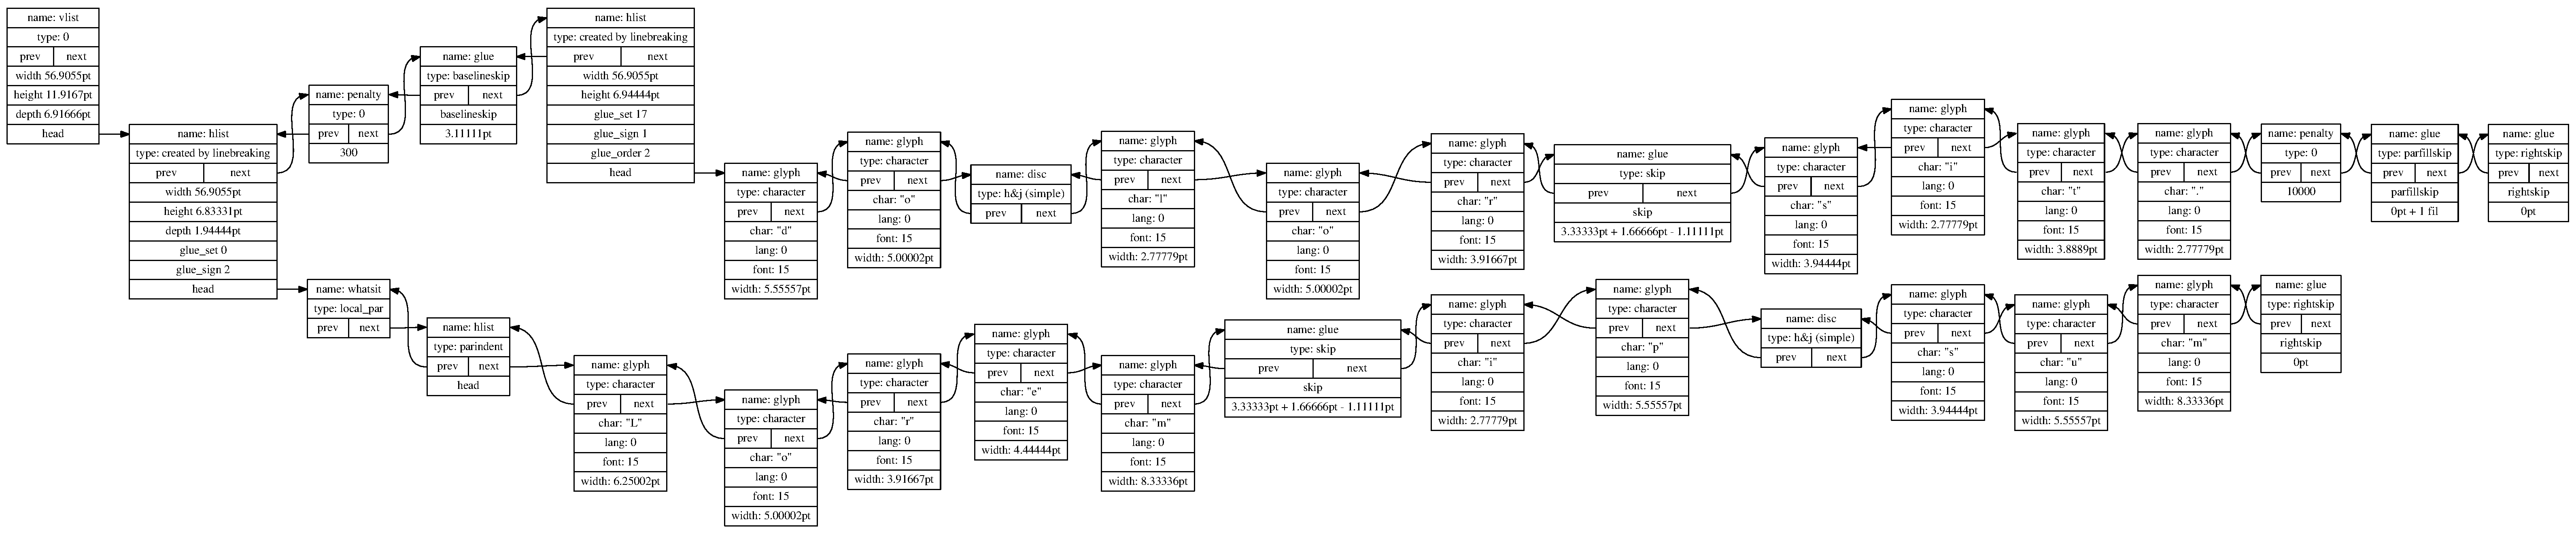
\includegraphics[width=\linewidth]{graphics/par}

\subsection{Tabular environment}

\noindent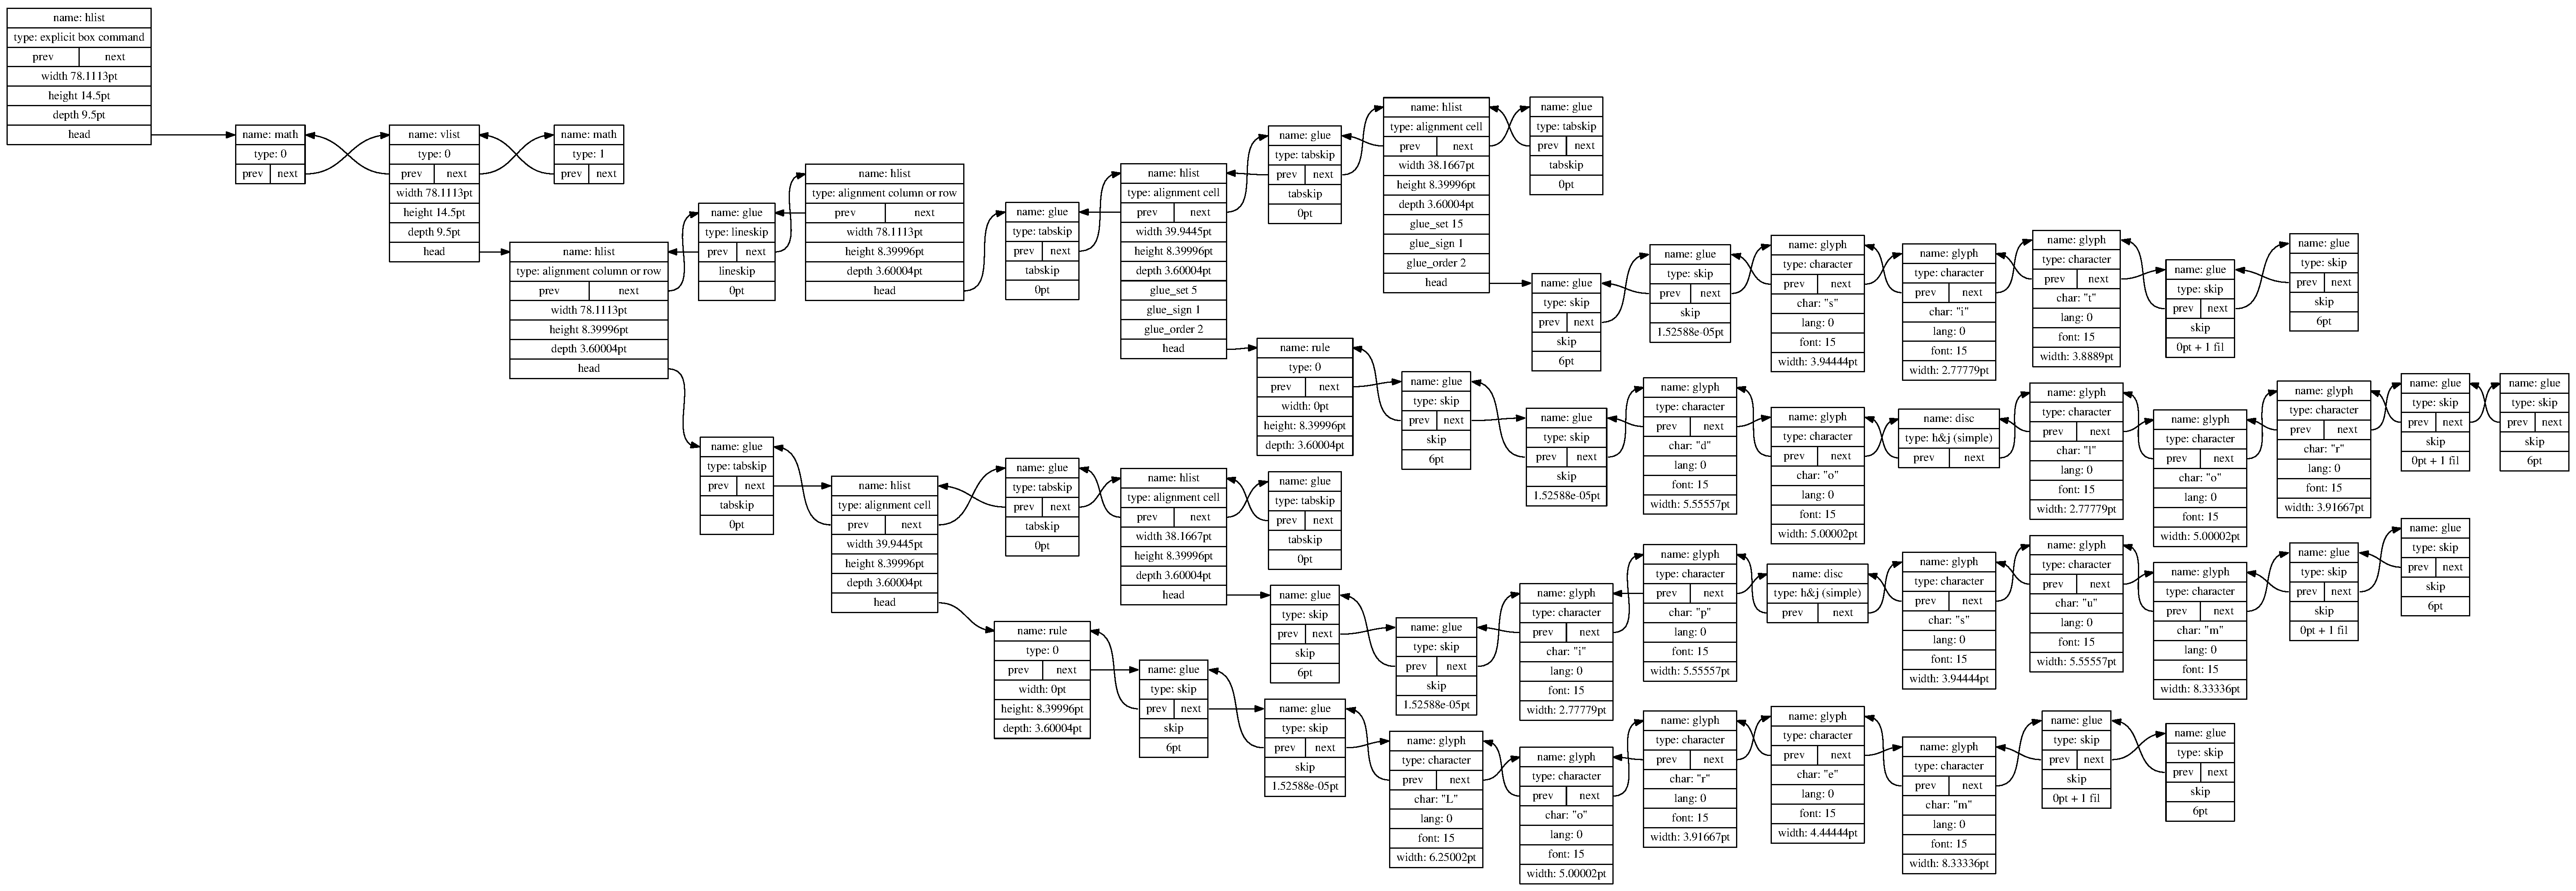
\includegraphics[width=\linewidth]{graphics/tabular}

\subsection{Picture environment}

\noindent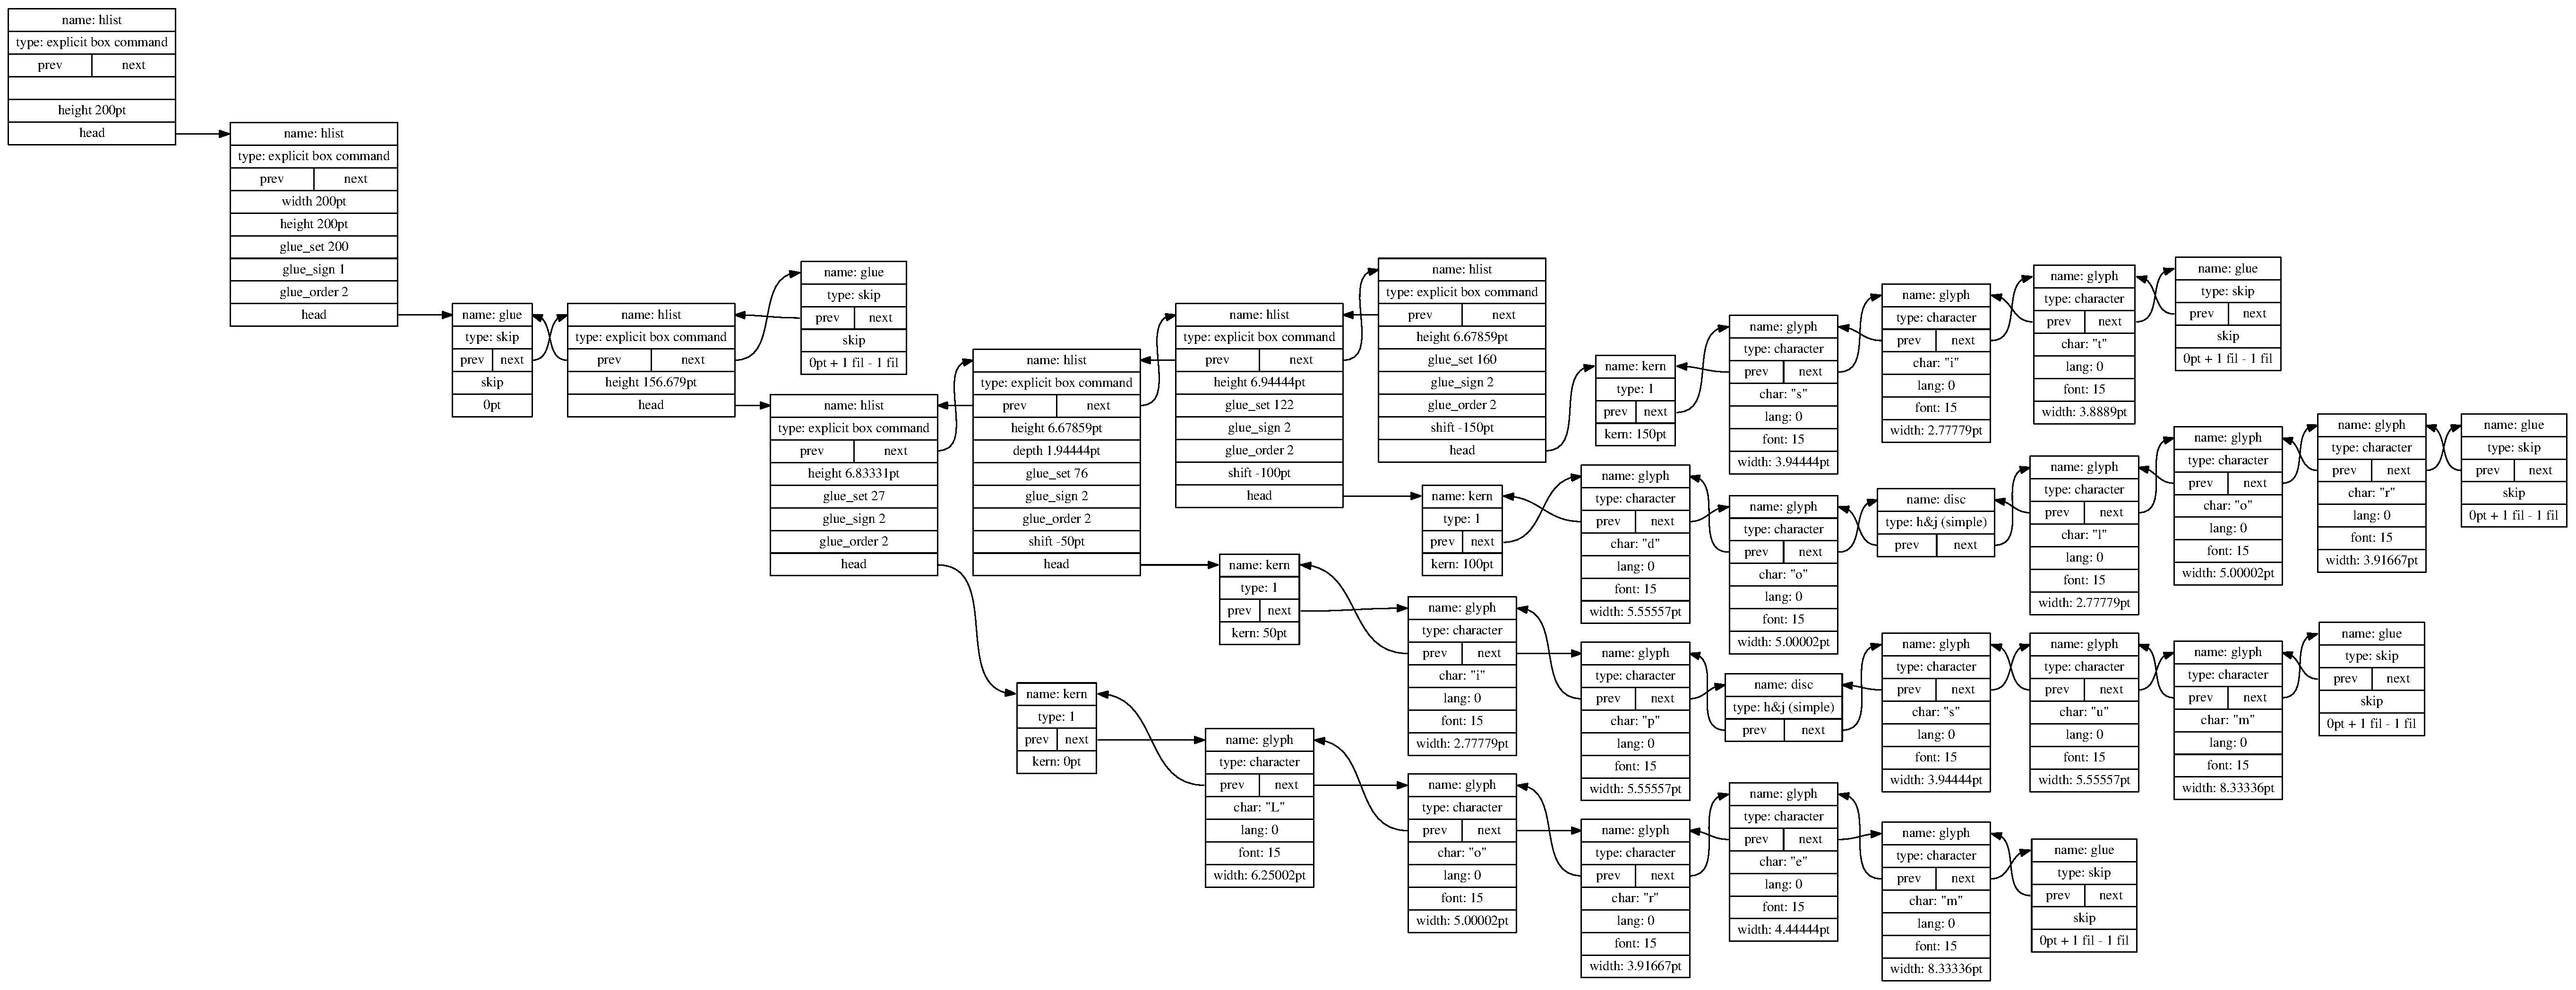
\includegraphics[width=\linewidth]{graphics/picture}

\DocInput{cloze.dtx}

\subsection{The file cloze.lua}

\inputminted{lua}{cloze.lua}

\pagebreak
\PrintChanges
\pagebreak
\PrintIndex
\end{document}
